%% LyX 1.2 created this file.  For more info, see http://www.lyx.org/.
%% Do not edit unless you really know what you are doing.
\documentclass[oneside,english]{amsart}
\usepackage[T1]{fontenc}
\usepackage[latin1]{inputenc}
\usepackage{graphicx}

\makeatletter

%%%%%%%%%%%%%%%%%%%%%%%%%%%%%% LyX specific LaTeX commands.
\providecommand{\LyX}{L\kern-.1667em\lower.25em\hbox{Y}\kern-.125emX\@}

%%%%%%%%%%%%%%%%%%%%%%%%%%%%%% Textclass specific LaTeX commands.
 \theoremstyle{plain}    
 \newtheorem{thm}{Theorem}[section]
 \numberwithin{equation}{section} %% Comment out for sequentially-numbered
 \numberwithin{figure}{section} %% Comment out for sequentially-numbered
 \newenvironment{lyxcode}
   {\begin{list}{}{
     \setlength{\rightmargin}{\leftmargin}
     \raggedright
     \setlength{\itemsep}{0pt}
     \setlength{\parsep}{0pt}
     \normalfont\ttfamily}%
    \item[]}
   {\end{list}}

\usepackage{babel}
\makeatother
\begin{document}

\vfill{}
\title{Intermediate Language for Code Generation and the ILCP API}
\vfill{}


\date{Feb 2003 }


\author{PaulCockshott}

\begin{abstract}
This describes the strategy of code generation to be used with the
ILCP code generator generator system for Pascal. It is intended to
be used by writers of compiler front ends. Familiarity with assembly
language and with compiler technology is assumed.
\end{abstract}
\maketitle

\section{What is ILCG}

ILCG is short for Intermediate Language for Code Generation. It is
a notation that serves two purposes:

\begin{enumerate}
\item It can be used to describe the semantics of a computer's instructionset.
\item It can be used to describe the semantics of a computer program.
\end{enumerate}
Like most formal notations it can have several concrete representations.
One representation would be as a flat ascii file using the grammar
defined in section \ref{sec:ILCG-grammar}. Another would be as an
internal tree structure in a computers memory. Tools and libraries
exist to translate flat ascii representations of ILCG into internal
tree structures based on the data-types of Java and Pascal. Since
this document is concerned with the use of compiler tools in Pascal
we shall concentrate on this representation.


\section{Structure of the code-generation process}

%
\begin{figure}
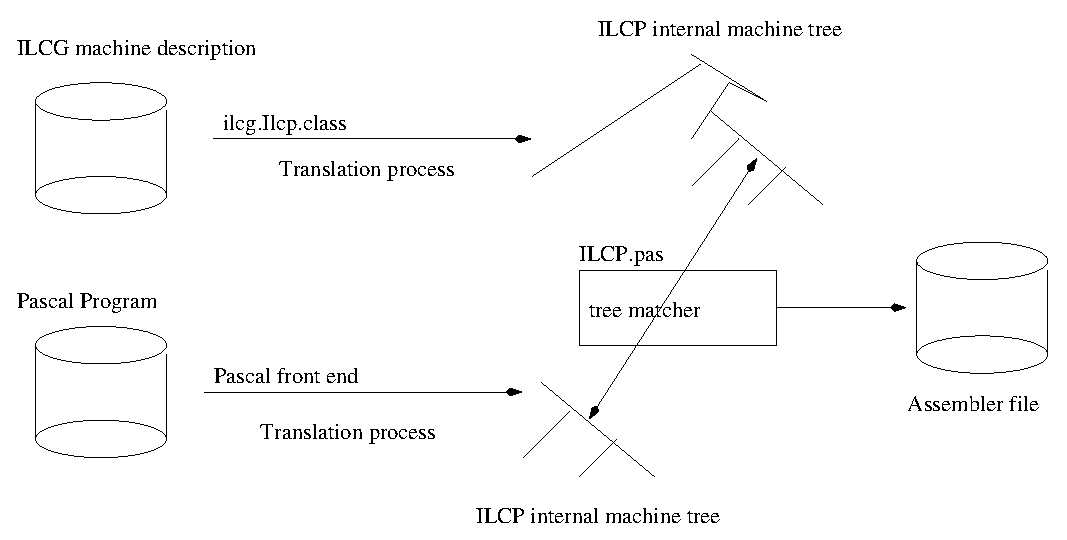
\includegraphics[  width=5in,
  keepaspectratio]{treediag}


\caption{Overview of the translation process\label{cap:Overview-of-the}}
\end{figure}


Figure \ref{cap:Overview-of-the} shows the way ILCG can be used to
translate high level languages into assembly code. Amachine description
in ILCG - for instance the 386 description given in section \ref{sec:Example-ILCG-machine},
is input to a translation program written in Java (\texttt{ilcg.Ilcp.java})
which generates a Pascal unit, which in this case we might call \texttt{I386.pas}.
When this unit is invoked during program startup it initialises a
collection of tables and trees which together constitute an internal
Pascal representation of the original Ascii machine description file.

A Pascal lexical and syntax analyser process a Pascal source file
and translate it to an internal Ilcp tree structure, with nodes of
type \texttt{ilcgnode}. The tree representing the program is then
compared to the tree representing the machine by a unit \texttt{Ilcp.pas}. 

Let us call the tree representing the machine $m$ and the tree representing
the program $p$. The tree matching unit takes each statement $s$
in $p$and searches for an instruction $i$ in $m$ which has the
same type signature. If the tree for the instruction $i$ and the
tree for the statement $s$ correspond exactly, then the corresponding
assembly instruction is output to an assembler file. If it does not
exactly correspond, the tree matcher attempts to break $s$ into a
series of substatement trees $s_{1},s_{2},...$ which can individually
be matched against instructions. 

This approach to machine code generation was pioneered by Susan Graham
in the 80s. It has the advantages of yielding very good matches between
the source code and the instructionset - matches which are frequently
as good as a human assembly coder could achieve. We will give an intial
example of how this works before going into more details


\subsection{Machine description files}

CPUs are defined in hardware description language ILCG. What follows
is a cut down example.


\subsection{Define registers}

\begin{verbatim}
*/
register int32 EAX assembles['eax'] ;
register int32 ECX assembles['ecx'] ;
register int32 EBX assembles['ebx'] ;
register word EBP assembles['ebp'] ;
alias register word FP = EBP(0:31) assembles ['ebp'];
reserved register word ESP assembles['esp'];
register int32 ESI assembles['esi'] ;
register int32 EDI assembles['edi'] ;
register int32 EDX assembles['edx'];
/*\end{verbatim}


\subsubsection{Define sets of registers}

\begin{verbatim}
*/
pattern indexreg means[EDI|ESI|EBX|EBP|ESP|EAX|EDX|ECX];
pattern accumulators means[EAX|EDX|ECX|EBX];
pattern ireg means [ indexreg] ;
pattern ureg means [EBP| ubx|udi|usi|udx|ESP|ucx|uax ] ;

pattern reg means [ireg|ureg];

/*\end{verbatim}


\subsubsection{Define operations supported}

\begin{verbatim}

*/
operation add means + assembles [ 'add'];
operation and means AND assembles[ 'and'];
operation or means OR assembles['or'];
operation xor means XOR assembles['xor'];/* */
operation sub means - assembles [ 'sub']; 
operation imul means * assembles ['imul '];
/*\end{verbatim}


\subsubsection{Define address modes}

\begin{lyxcode}
pattern~labelf(label~l)~\\
~means~{[}l{]}~\\
~assembles{[}l{]};~\\
~\\
pattern~constf(signed~s)~\\
~means{[}const~s{]}~\\
~assembles~{[}s{]};~\\
pattern~offset~means{[}constf|labelf{]};~\\
pattern~regindirf(reg~r)~~\\
~means{[}\textasciicircum{}(r)~{]}~\\
~assembles{[}~r~{]};

pattern~baseplusoffsetf(reg~r,~offset~s~)~\\
~means{[}+(~\textasciicircum{}(r)~,~s){]}~\\
~assembles{[}~r~'+'~s~{]};~\\
\begin{verbatim} 
pattern eaform means[
 labelf|
 basePlusScaledIndexPlusOffsetf| 
 baseplusoffsetf  ];
\end{verbatim}
\end{lyxcode}

\subsubsection{Type casts}

The syntax for the type casts is C style so we have for example \texttt{(ieee64)
int32} to represent a conversion of an 32 bit integer to a 64 bit
real. These type casts act as constraints on the pattern matcher during
code generation. They do not perform any data transformation. They
are inserted into machine descritions to constrain the types of the
arguments that will be matched for an instruction. They are also used
by compilers to decorate ILCG trees in order both to enforce, and
to allow limited breaking of, the type rules.


\subsubsection{Define instructions}

An instruction format is an abstraction over a class of concrete instructions.
It abstracts over particular operations and types thereof whilst specifying
how arguments can be combined.

\begin{lyxcode}
\textbf{instruction~pattern~LOAD(maddrmode~rm,~anyreg~r1,~wordupto32~t)~}~\\
~\textbf{means{[}~(ref~t)~r1:=~(t)\textasciicircum{}(rm~){]}~}~\\
~\textbf{assembles{[}'mov~'~r1~','~t~'~'~rm{]};}~

\textbf{instruction~pattern~STORER(maddrmode~rm,~reg~r1,~word32~t)}~\\
~\textbf{means{[}~(ref~t)~rm:=~\textasciicircum{}(~r1)~{]}}~\\
~\textbf{assembles{[}'mov~'~t~'~'rm','~r1{]};}~\\
\textbf{}~\\
\textbf{instruction~pattern~STORELIT(addrmode~rm,~type~t,~int~s)}~\\
~\textbf{means{[}~(ref~t)~rm:=~(t)const~s~{]}}~\\
~\textbf{assembles{[}'mov~'~t~'~'rm~','~'~'~s{]};}
\end{lyxcode}

\paragraph*{Arithmetic instructions}

\begin{lyxcode}
\textbf{instruction~pattern~}

~\textbf{RRM(operator~op,~reg~r1,~maddrmode~rm,~int~t)}

~\textbf{means~{[}r1:=(t)~op(~$\uparrow $((ref~t)r1),$\uparrow $((ref~t)~rm)){]}}

~\textbf{assembles{[}op~'~'~r1~','~rm~{]}~;}

\textbf{instruction~pattern~}

~\textbf{RR(~operator~op,~anyreg~r1,~anyreg~r2,~int~t)}

~\textbf{means{[}r1:=(t)~op(~$\uparrow $((ref~t)~r1),$\uparrow $((ref~t)~r2)){]}}

~\textbf{assembles{[}op~'~'~r1~','~r2{]};}
\end{lyxcode}
The \textbf{int t} parameter is a type variable which will match any
integer type - this stops the instructions from being used for floating
point operations

\begin{lyxcode}
\textbf{instruction~pattern~RMLIT(nonmultoperator~op,}~\\
~\textbf{~~~~~~~~~~~~~~~~~~~~~addrmode~rm,~type~t,~offset~sm)}~\\
~\textbf{means{[}~(ref~t)~rm:=~op(\textasciicircum{}(rm),(t)~sm)~{]}}~\\
~\textbf{assembles{[}op~'~'~t~'~'~rm~','~sm{]};}~\\
\textbf{}~\\
\textbf{instruction~pattern~INC(addrmode~rm,int~t)}~\\
~\textbf{means{[}(ref~t)rm:=~+~(\textasciicircum{}(rm),1){]}}~\\
~\textbf{assembles{[}'inc~'~t~'~'~rm{]};}~\\

\end{lyxcode}

\subsubsection{Define instruction order}

\begin{lyxcode}
instructionset{[}LOAD|~STORELIT|~INC|~RMLIT|~RRM|~RR|~STORE{]};
\end{lyxcode}
List these from the most specific to the most general 

Store is most general, since it can store the result of any expression
that has been evaluated to a register. Load is the most specific,
as it is only used in the middle of expression evaluation and can
only match a variable.


\subsection{Matching}

Source trees are matched against the machine description by a function
within the unit \texttt{ILCP.pas}:

\begin{lyxcode}
function~match(m:pilcgnode;var~b:rollbackbuffer):boolean;
\end{lyxcode}
For each instruction pattern in turn try to match the \textbf{m} to
the meaning of the instruction, if a match is found output the assembler
part substituting in the parameters where relevant, otherwise return
false.

In doing this the following substitutions can be made

\begin{enumerate}
\item for a register parameter r and expression e, recursively call match(r:=e)
\item for an address mode parameter m , and expression e attempt to match
the address mode to e.
\end{enumerate}

\paragraph*{Example}

i:=2

Assume i at offset 10 from ebp, parser generates the tree shown in
figure \ref{cap:Tree-for-x:=3D2}.

%
\begin{figure}
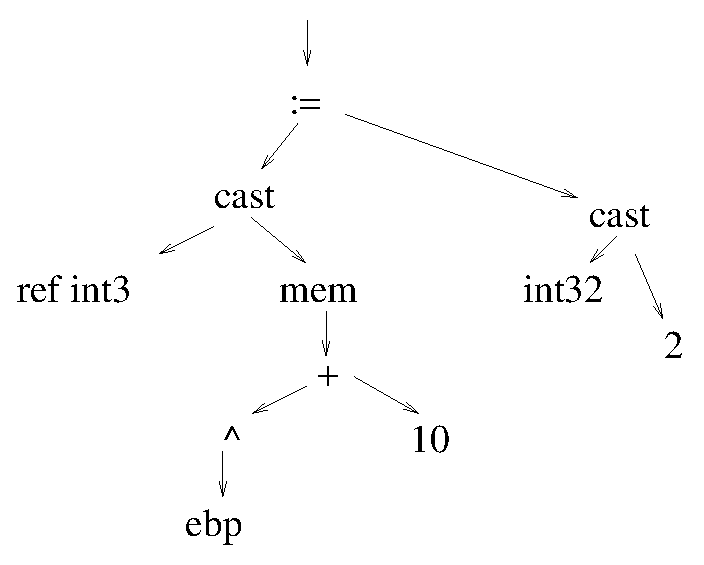
\includegraphics[  height=2in,
  keepaspectratio]{assntree}


\caption{Tree for i:=2 where i is at offset 10 from ebp\label{cap:Tree-for-x:=3D2}}
\end{figure}


we can represent this textually as

\emph{(ref int32)mem(+(\textasciicircum{}(ebp),10)):= (int32)2}

match this to

\textbf{(ref t) r1:= (t)\textasciicircum{}(rm ) : LOAD}

\textbf{(ref t) rm:= (t)const s : STORELIT}

\textbf{(ref t)rm:= + (\textasciicircum{}(rm),1) : INC}

\textbf{(ref t) rm:= op(\textasciicircum{}(rm),(t) sm) : RMLIT}

\textbf{r1:=(t) op( \textasciicircum{}((ref t)r1),\textasciicircum{}((ref
t) rm)) :RRM}

\textbf{(ref t) rm:= \textasciicircum{}( r1) : STORER}

try LOAD, first bind \textbf{t} to \emph{int32}, then attempt to bind
\textbf{r1} to \emph{mem(+(\textasciicircum{}(ebp),10))} this fails
because \textbf{r1} is of type register

try STORELIT, bind \textbf{t} to \emph{int32} then attempt to bind
\textbf{rm} to \emph{mem(+(\textasciicircum{}(ebp),10))}

rm is of type addrmode defined by

\begin{lyxcode}
\textbf{pattern~addrmode~means{[}maddrmode|anyreg{]};}

\textbf{pattern~maddrmode(eaform~f)~means{[}mem(f)~{]}~}

~\textbf{assembles{[}~'{[}'~f~'{]}'~{]}};
\end{lyxcode}
Try to match maddrmode to \emph{mem(+(\textasciicircum{}(ebp),10))
,} \textbf{mem(f)}\emph{,} this works if f binds to +(\textasciicircum{}(ebp),10).

But a valid eaform is the pattern

\begin{lyxcode}
pattern~baseplusoffsetf(reg~r,~offset~s~)~\\
~means{[}+(~\textasciicircum{}(r)~,~s){]}~\\
~assembles{[}~r~'+'~s~{]};
\end{lyxcode}
which clearly matches.

We have now matched

(ref int32) mem(+(\textasciicircum{}(ebp),10)):=

we have to match 2 to const s - which obviously works

Then generate the assembler pattern for storelit

\begin{lyxcode}
\textbf{{[}'mov~'~t~'~'rm~','~'~'~s{]}}
\end{lyxcode}
substituting in the parameters

t->int32->'dword'

rm->memaddrword->eaform->baseplus offset-> '{[}ebp+10{]}'

s->2

so we generate

\begin{lyxcode}
mov~dword{[}ebp+10{]},2
\end{lyxcode}
which is the optimal instruction for the instructionset.


\subsection{Other optimisations}

In addition to matching statements against instructions the unit ilcp.pas
performs some other optimisations.


\subsubsection{Constant Folding}

One frequently has expressions all of part of which can be computed
at compile time. These arise both because of constants the user has
introduced and also in the evaluation of array expressions.

Example

\begin{lyxcode}
const~a=9;

const~b=1;

var~c:Integer~;

begin

~c:=getint;

~c:=c+a{*}b;
\end{lyxcode}
Visual inspection shows that the last line could read 

\begin{lyxcode}
c:=c+9~
\end{lyxcode}
Consider the formula

(7+a)+(b+5) with a, b both variables not constants

This has tree

\begin{lyxcode}
~~~~~~~+

~~~~~~~|

~~~-{}-{}-{}-{}-{}-{}-{}-{}-{}-{}-{}-{}-{}-{}-{}-{}-{}-

~~~|~~~~~~~~~~~~~~~~|

~~~+~~~~~~~~~~~~~~~~+

~~~|~~~~~~~~~~~~~~~~|

-{}-{}-{}-{}-{}-{}-{}-{}-~~~~~~~~-{}-{}-{}-{}-{}-{}-{}-{}-{}-{}-{}-

|~~~~~~~|~~~~~~~|~~~~~~~~~~~~|

7~~~~~~~a~~~~~~~b~~~~~~~~~~~~5
\end{lyxcode}
As it stands it can not be evaluated as a,b stop both branches of
the tree from being known at compile time. But we know that in principle
it is equal to a+b+12. To get this we must re-organise the tree. 

The strategy is to first move all the constant nodes to the right
hand side of the tree leaving the variables on the left.

The tree now becomes

\begin{lyxcode}
~~~~~~~+

~~~~~~~|

~~~-{}-{}-{}-{}-{}-{}-{}-{}-{}-{}-{}-{}-{}-{}-{}-{}-{}-

~~~|~~~~~~~~~~~~~~~~|

~~~+~~~~~~~~~~~~~~~~+

~~~|~~~~~~~~~~~~~~~~|

-{}-{}-{}-{}-{}-{}-{}-{}-~~~~~~~~-{}-{}-{}-{}-{}-{}-{}-{}-{}-{}-{}-

|~~~~~~~|~~~~~~~|~~~~~~~~~~~~|

a~~~~~~~7~~~~~~~b~~~~~~~~~~~~5
\end{lyxcode}
We next promote any constant right hand sides.      That is to say

we raise them to the right. After one stage we get:

\begin{lyxcode}
~~~~~~~~~~~~~+

~~~~~~~~~~~~~|

~~~~~~~~-{}-{}-{}-{}-{}-{}-{}-{}-{}-

~~~~~~~|~~~~~~~~~~|

~~~~~~~+~~~~~~~~~~+

~~~~~~~|~~~~~~~~~~|

~~~~~~~a~~~~~~~-{}-{}-{}-{}-{}-{}-{}-{}-{}-{}-{}-{}-

~~~~~~~~~~~~~~~|~~~~~~~~~~~|

~~~~~~~~~~~~~~~+~~~~~~~~~~~7

~~~~~~~~~~~~~~~|

~~~~~~~~~~~-{}-{}-{}-{}-{}-{}-{}-{}-{}-{}-{}-

~~~~~~~~~~|~~~~~~~~~~~~|

~~~~~~~~~~b~~~~~~~~~~~~5
\end{lyxcode}
We next recursively evaluate the re-organised tree.

This will again attempt to reorganise:

\begin{lyxcode}
~~~~~~~~~~~~~+

~~~~~~~~~~~~~|

~~~~~~~~-{}-{}-{}-{}-{}-{}-{}-{}-{}-

~~~~~~~|~~~~~~~~~~|

~~~~~~~+~~~~~~~~~~+

~~~~~~~|~~~~~~~~~~|

~~~~~~~a~~~~~~~-{}-{}-{}-{}-{}-{}-{}-{}-{}-{}-{}-{}-

~~~~~~~~~~~~~~~|~~~~~~~~~~~|

~~~~~~~~~~~~~~~b~~~~~~~~~~~+

~~~~~~~~~~~~~~~~~~~~~~~~~~~|

~~~~~~~~~~~~~~~~~~~~~-{}-{}-{}-{}-{}-{}-{}-{}-{}-{}-{}-

~~~~~~~~~~~~~~~~~~~~|~~~~~~~~~~~~|

~~~~~~~~~~~~~~~~~~~~7~~~~~~~~~~~~5
\end{lyxcode}
which can be evaluated to a+b+12


\subsubsection{Identity Element}

A value $\varepsilon $ is the identity element of a typed operator
$\otimes $ if

x $\otimes $$\varepsilon $= x , $\forall $x

Then for we have the following typical identity elements:

\begin{center}\begin{tabular}{|c|c|c|}
\hline 
type&
operator&
value\\
\hline
\hline 
number&
+&
0\\
\hline 
number&
{*}&
1\\
\hline 
bool&
or&
false\\
\hline 
bool&
and&
true\\
\hline
\end{tabular}\end{center}

A constant folder should thus apply the following transformations

x + 0 $\Rightarrow $x

x {*} 1 $\Rightarrow $x

x - 0 $\Rightarrow $x

x / 1 $\Rightarrow $x

x or false $\Rightarrow $x

x and true $\Rightarrow $x

x xor false $\Rightarrow $x

Note that these apply even when x not known till run time


\subsubsection{Absorbers}

A value $\alpha $ is the absorber of a typed operator $\otimes $
if

x $\otimes $$\alpha $= $\alpha $ , $\forall $x

The absorbers relevant for compilation are

\begin{center}\begin{tabular}{|c|c|c|}
\hline 
type&
operator&
value\\
\hline
\hline 
number&
{*}&
0\\
\hline 
bool&
and&
false\\
\hline 
bool&
or&
true\\
\hline
\end{tabular}\end{center}

thus a constant folder should handle the operations

x {*} 0 $\Rightarrow $0

x and false $\Rightarrow $false

x or true $\Rightarrow $true


\subsubsection{Dead Code Removal}

This is a special instance of constant folding. Consider the following:

\begin{lyxcode}
const~a=9;

begin

~~if~a>12~then~c:=4~else~c:=3;

end;
\end{lyxcode}
We know from inspection that a is never >12 so that the then part
of the if-then-else is never taken. So we can rewrite this as:

\begin{lyxcode}
const~a=9;

begin

~~~c:=3;

end;
\end{lyxcode}
We do this by extending the constructor function for if-then-else
so that if the condition is known at compile time only one branch
of the loop is returned.


\subsubsection{Register caching of induction variables}

Inner loops which have no function calls have their loop induction
variables replaced by registers.


\subsubsection{Vectorisation}

Most modern PCs are capable of performing several arithmetic operations
in parallel. For instance a P4 can add 4 32 bit floating point operations
in a single instruction, an AMD machine can add 2 32 bit floats with
one instruction. The code generator analyses inner loops and those
which have the general form

\begin{lyxcode}
for~i:=low~to~high~do~

~~a{[}i{]}:=~b{[}i{]}~op1~c{[}i{]}~op2~d{[}i{]}~....
\end{lyxcode}
are vectorised if vector instructions to perform operations op1, op2
etc exist.

The resulting code takes the form of two loops, the quotient loop
and the remainder loop. The quotient loop is executed in parallel
up to the parallism factor defined by the machines vector registers,
the remainder loop is then serialised.

Suppose low=0 and high =10 and the type of a{[}i{]},b{[}i{]} etc is
32 bit float and that the machine is p4, then the quotient loop translates
to

\begin{lyxcode}
for~i:=~0~to~7~step~4~do

a{[}i..i+3{]}:=b{[}i..i+3{]}~op1~c{[}i..i+3{]}~op2~d{[}i..i+3{]}~....
\end{lyxcode}
the remainder loop translates to

\begin{lyxcode}
for~i:=8~to~10~do~

~~a{[}i{]}:=~b{[}i{]}~op1~c{[}i{]}~op2~d{[}i{]}~....
\end{lyxcode}
The absence of scalar to vector arithmetic instructions on the Intel
and AMD processors means that the gains from vectorisation are more
limited if any of the operands in the assignment statement are scalars
rather than vectors. The code generator will attempt to vectorise
these, but in doing so it is forced to make multiple copies of scalars
prior to loading them into vector registers. This is relatively costly.

\begin{lyxcode}

\end{lyxcode}

\subsubsection{Dead for loop elimination}

given

\begin{lyxcode}
for~i\textasciitilde{}~e1~..~e2~do~c1
\end{lyxcode}
then if we know at compile time that e1 will always be greater than
e2, we can remove the entire for statement.


\subsubsection{Loop unrolling}

It is advantageous to unroll loops to some degree. Unrolling loops
has the advantages that:

\begin{enumerate}
\item Since the size of basic block is increased the chances of pipeline
stalls are reduced. This may be less significant with the very latest
processors.
\item The total number of instructions executed can be reduced since in
simple an inner loop the comparison and branch instructions can make
up around 30\% of the instructions executed. If we perform 5 fold
unrolling we reduce this overhead, allowing the loop to execute about
25\% faster.
\end{enumerate}
A for loop of the form

\begin{lyxcode}
for~i:=~1~to~10~do~x{[}i{]}:=j{[}i{]}+1;
\end{lyxcode}
Will be expanded to

\begin{lyxcode}
for~i:=1~to~10~do~begin

~x{[}i{]}:=j{[}i{]}+1;

~i:=i+1;

~x{[}i{]}:=j{[}i{]}+1;

~i:=i+1;

~x{[}i{]}:=j{[}i{]}+1;

~i:=i+1;

~x{[}i{]}:=j{[}i{]}+1;

~i:=i+1;

~x{[}i{]}:=j{[}i{]}+1;

end
\end{lyxcode}
Shorter loops are expanded less agressively. For loops of length less
than 5, this enables the loop to be replaced with straight line code.


\subsubsection{Unitary loop handling}

In the loop

\begin{lyxcode}
for~i\textasciitilde{}~\textsl{e1}~..~\textsl{e2}~do~\textsl{c1}
\end{lyxcode}
If we know that \texttt{\textsl{e1=e2}}, then we can substitute it
with

\begin{lyxcode}
i:=\textsl{e1};\textsl{c1};
\end{lyxcode}
So that 

\begin{lyxcode}
const~x=3~;

~~~~y=3-x;

begin

~~for~i\textasciitilde{}1~to~y+1~do~x{[}i{]}:=~z{[}i{]}+y;

end;
\end{lyxcode}
will simplify to

\begin{lyxcode}
i:=1~;~x{[}i{]}:=z{[}i{]};
\end{lyxcode}
Since vectorisation and loop unrolling are performed prior to dead
loop removal and unitary loop handling the net effect is that

\begin{enumerate}
\item Single precision floating point loops of length up to 20 are replaced
with vectorised straight line code.
\item Byte loops of length up to 40 are replaced by vectorised straight
line code.
\item For loops whose length modulo the vector register length is zero,
the remainder loop is ellided, giving a fully vectorised loop.
\end{enumerate}

\section{ILCG nodes and their semantics}


\subsection{Types in ILCG}

ILCG is a strongly typed notation. Expression trees, memory locations
and registers all have types. The type system is relatively simple
being made up of base types and fixed length vectors of these types.
Whilst less flexible than the type system of high level languages
this is sufficient to describe the types understood by current CPUs.


\subsubsection{Base types}

Base types are subdivided into integer, real, and unformated types.
Real types are further subdivided according to whether they are signed
or not, and according to length. Table \ref{cap:The-base-types} ,
sumarises the base types supported.

%
\begin{table}

\caption{The base types of ILCG\label{cap:The-base-types}}

\begin{tabular}{|c|c|c|}
\hline 
Name&
length in bits&
category\\
\hline
\hline 
octet&
8&
untyped format\\
\hline 
halfword&
16&
untyped format\\
\hline 
word&
32&
untyped format\\
\hline 
doubleword&
64&
untyped format\\
\hline 
quadword&
128&
untyped format\\
\hline
\hline 
int8&
8&
signed integer\\
\hline 
int16&
16&
signed integer\\
\hline 
int32&
32&
signed integer\\
\hline 
int64&
64&
signed integer\\
\hline
\hline 
uint8&
8&
unsigned integer\\
\hline 
uint16&
16&
unsigned integer\\
\hline 
uint32&
32&
unsigned integer\\
\hline
\hline 
ieee32&
32&
floating point\\
\hline 
ieee64&
64&
floating point\\
\hline
\end{tabular}
\end{table}



\subsubsection{Reference types}

A base type describes a unitary value. A storage location such as
a register or a memory word is a reference type. A register that contains
a 32 bit signed integer is of type \textbf{ref int32} for example.
Conceptually this is because the register refers to one of the integers,
a usage borrowed from Algol-68 to distinguish permisible operations
on storage locations from those permisable on simple values.


\subsubsection{Vector types}

Avector type can be formed from a base type, hence we can have a type
like \textbf{vector(4) ieee32} to represent a vector of four single
precision floating point values. The vector definition facility is
limited to fixed length vectors of base types, two dimensional arrays
are not supported. This is obviously less sophisticated than a high
level programming language requires but is sufficient to describe
the types that can be manipulated by the vector registers of current
machines.


\subsubsection{Pascal encoding}

In the ILCG trees manipulated by Pascal programs the types of values
are encoded in format tag words as shown in figure \ref{cap:Layout-of-a}.
Since the type system is finite, a single word rather than a tree
structure suffices. 

If only the length field of the word is initialised, then the word
indicates an untyped format. 

The use of the integer and real bits in the word are mutually exclusive.
The signed bit should only be used if the integer bit is set. 

The vector length field should only be used if the vector bit is set.

A collection of formats are exported as predeclared constants from
ilcp.pas: \texttt{fint, fint16, fuint16} etc.

%
\begin{figure}
\begin{center}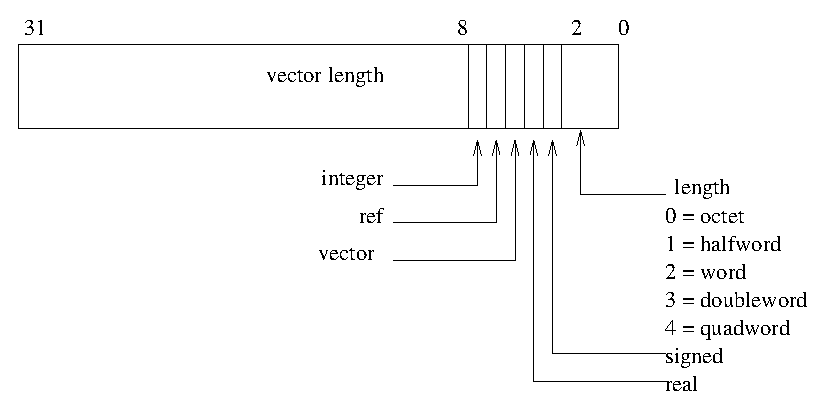
\includegraphics[  width=4in]{typetag}\end{center}


\caption{Layout of a format description word in an ILCG tree\label{cap:Layout-of-a}}
\end{figure}



\subsection{ILCG tree nodes}

The nodes of the ILCG internal tree are represented by variant records
in Pascal with a tag field of the type:

\begin{lyxcode}
nodeclass=(

~deref,~~~arraysubscript,reallit,~~~~~~intlit,

~format,~~regstack,~~~~~~unboundformat,ref,

~gotonode,patterntag,~~~~failure,~~~~~~typevar,

~Assignop,forloop,~~~~~~~memref,~~~~~~~dyadicop,

~ifnode,~~sequence,~~~~~~alternation,~~monad,

~monop,~~~dyad,~~~~~~~~~~typecast,~~~~~constant,

~param,~~~reg,~~~~~~~~~~~location,~~~~~labelnode,

~procedurenode

);
\end{lyxcode}
Many of these sorts of nodes are used only in machine descriptions.
The format of the variant records describing the nodes in Pascal is:

\begin{lyxcode}
ilcgnode=~record

~~~~~~simple:boolean;~\{~~already~simplified~\}

~~~~~~case~tag:nodeclass~of

~~~~~~patterntag:(pat:ppattern;);



~~~~~~deref,ref,constant,monad,

~~~~~~dyad,memref,typecast,failure:

~~~~~~~(arg,fn,arg2:pilcgnode;);



~~~~~~location:(locvalue:pilcgnode;);



~~~~~~regstack:(stackdetails:registerstack;);



~~~~~~arraysubscript:

~~~~~~~~(~base,~\{~base~address~\}

~~~~~~~~~~offset:pilcgnode;~\{~i,th~element~\}

~~~~~~~~~~\{~step~calculated~from~format\}

~~~~~~~~~~elementformat:integer);



~~~~~~Assignop,gotonode:

~~~~~~~(src,dest:pilcgnode;);



~~~~~~alternation:

~~~~~~~(first,last:integer);



~~~~~~intlit,reallit:

~~~~~~~(~reallitarg:intreal;

~~~~~~~~~intlitarg:intint;

~~~~~~~~~litformat:integer);



~~~~~~ifnode:

~~~~~~~(~condition,

~~~~~~~~~action,

~~~~~~~~~alternative:pilcgnode;);



~~~~~~unboundformat,format:

~~~~~~~(formatarg:integer);



~~~~~~monop,dyadicop:

~~~~~~~(opname:string{[}15{]};);



~~~~~labelnode,param,reg:

~~~~~~~(index:integer;);



~~~~~sequence:

~~~~~~~(current,next:pilcgnode;);



~~~~~forloop:

~~~~~~(~indexvar,

~~~~~~~~start,

~~~~~~~~stop,

~~~~~~~~incr,

~~~~~~loopaction:pilcgnode);



~~~~~~procedurenode:

~~~~~~~(~procedurebody:pilcgnode;

~~~~~~~~~languagespecificinfo:pointer);

end;
\end{lyxcode}

\subsection{Constructor functions}

Many of these classes of nodes can only occur in machine description
trees, but for the ones that are used in constructing program trees,
a collection of constructor functions is exported by the unit \texttt{ILCP.pas}.function
I shall describe the semaintics of the ILCG trees in terms of these
constructor functions.


\subsubsection{new\_arraysubscript}

\begin{lyxcode}
function~new\_arraysubscript(baseaddr,index:pilcgnode;form:integer):pilcgnode;
\end{lyxcode}
Creates a node representing an array subscription operation. The baseaddr
should be an ILCG tree for an integer expression giving the starting
address of the array. The index should be a tree giving an ILCG expression
for the offset into the array. The form parameter is a tag word describing
the format of the array elements ( not the array itself ). The base
address should be adjusted to allow for arrays starting at non-zero
values. 


\paragraph*{Example: }

given the pascal array declaration:

var x:array{[}2..4{]} of integer; i:integer;

then if x was at address 100 and i at address 90, then the subscription
\texttt{x{[}i{]}} would translate to the ILCG tree

\begin{lyxcode}
new\_arraysubscript(

~new\_intlit(100-8,fint32),~~~~~\{~allow~for~starting~at~2~\}

~new\_deref(new\_memref(new\_intlit(90,fint32),fint32)),

~fint32);
\end{lyxcode}

\subsubsection{new\_assign}

\begin{lyxcode}
function~new\_assign(dest,src:pilcgnode):pilcgnode;~
\end{lyxcode}
This creates a pointer to an ilcgnode whose tag is \texttt{assignop}.
The source should be a tree of type \textbf{ref} \emph{t} and the
destination a tree of type \emph{t}. The effect when passed to the
code generator is to generate code to evaluate the \texttt{src} and
store it in the \texttt{dest}.


\subsubsection{new\_deref}

\begin{lyxcode}
function~new\_deref(loc:pilcgnode):pilcgnode;~
\end{lyxcode}
This creates a node representing the memory or register dereferencing
operation. If \texttt{x} is a node representing a location, \texttt{new\_deref(x)}
is a node representing fetching the contents of a location. Thus if
\texttt{x,y} are both registers or memory locations \texttt{new\_assign(x,new\_deref(y))}
represents the operation of copying the contents of \texttt{y} into
\texttt{x}, or in pascal source terms \texttt{x:=y}.

%
\begin{table}

\caption{Monadic operations.\label{cap:Monadic-operations.}}

\begin{center}\begin{tabular}{|c|l|l|}
\hline 
operator&
means&
comment\\
\hline
\hline 
'EXTEND'&
extend precision&
expand a short integer rep to longer rep\\
\hline 
'POP'&
pop off stack&
argument must be a stack\\
\hline 
'NOT'&
bitwise negate&
\\
\hline 
'SQRT'&
squareroot&
returns a real\\
\hline 
'ROUND'&
round to integer&
argument must be real\\
\hline 
'COS'&
cosine&
\\
\hline 
'SIN'&
sine&
\\
\hline 
'TAN'&
tangent&
\\
\hline 
'ABS'&
absolute value&
\\
\hline 
'FLOAT'&
float an integer&
\\
\hline 
'LN'&
natural log&
\\
\hline
\end{tabular}\end{center}

\begin{lyxcode}
~\end{lyxcode}

\end{table}



\subsubsection{new\_dyad}

\begin{lyxcode}
function~new\_dyad(left:pilcgnode;op:string;right:pilcgnode):pilcgnode;~
\end{lyxcode}
This creates a node representing a binary expression. The operators
are drawn from the set of strings shown in table \ref{cap:Dyadic-operators}.


\paragraph*{Example}

\begin{lyxcode}
new\_assign(x,~new\_dyad(new\_deref(x),'+',~new\_deref(y)));
\end{lyxcode}
%
\begin{table}
\begin{lyxcode}

\end{lyxcode}

\caption{Dyadic operators\label{cap:Dyadic-operators}}

\begin{lyxcode}
\begin{center}\begin{tabular}{|c|l|l|}
\hline 
string&
means&
comment\\
\hline
\hline 
'{*}'&
multiply&
\\
\hline 
'AND'&
bitwise and&
\\
\hline 
'/'&
divide&
\\
\hline 
'PUSH'&
push on stack&
left arg must be a stack\\
\hline 
'OR'&
bitwise or&
\\
\hline 
'+'&
add&
\\
\hline 
'MIN'&
return least&
\\
\hline 
'MAX'&
return greater&
\\
\hline 
'-'&
subtract&
\\
\hline 
'REP'&
replicate&
a REP $n$makes an $n$ element vector or a\\
\hline 
'='&
equals&
by default returns byte with true = FF\\
\hline 
'<>'&
not equals&
\\
\hline 
'>='&
greater than or equal&
\\
\hline 
'<='&
less than or equal&
\\
\hline 
'>'&
greater than&
\\
\hline 
'<'&
less thean&
\\
\hline 
'>\,{}>'&
shift right&
a>\,{}>n shifts a n places right\\
\hline 
'<\,{}<'&
shift left&
\\
\hline 
'{*}:'&
saturated multiply&
\\
\hline 
'-:'&
saturated subtract&
\\
\hline 
'+:'&
saturated add&
\\
\hline 
'CALL'&
call procedure&
x CALL y, x is procedure, y arglist\\
\hline 
'MOD'&
remainder&
\\
\hline
\end{tabular}\end{center}\end{lyxcode}

\end{table}



\subsubsection{new\_monad}

\begin{lyxcode}
function~new\_monad(op:string;right:pilcgnode):pilcgnode;
\end{lyxcode}
This creates a node representing the application of a monadic operator.

The monadic operators are drawn from the set shown in table \ref{cap:Monadic-operations.}.
They are typically operations for which hardware support exists and
for which subroutines calls are not necessary.


\subsubsection{new\_for}

\begin{lyxcode}
function~new\_for(~indexvar,~start,~stop,~incr,~loopaction:pilcgnode):pilcgnode;~
\end{lyxcode}
Generates a new for loop tree, equivalent to:

\begin{lyxcode}
for~indexvar:=start~to~stop~step~incr~do~loopaction.
\end{lyxcode}
The value of the indexvar is undefined on exit from the loop. For
loops are the target for vectorisation optimisations. Loops that use
explicit gotos will not be vectorised.


\subsubsection{new\_format}

\begin{lyxcode}
function~new\_format(form:integer):pilcgnode;~
\end{lyxcode}
Given an ILCG type tag (see fig \ref{cap:Layout-of-a}), this creates
an ILCG node that can be used in a typecast.


\paragraph*{Example: }

\begin{lyxcode}
new\_format(fint32);
\end{lyxcode}

\subsubsection{new\_goto}

\begin{lyxcode}
function~new\_goto(dest:pilcgnode):pilcgnode;
\end{lyxcode}
Creates a node representing a branch. The destination can be a label
or an expression that evaluates to an address.


\subsubsection{new\_if}

\begin{lyxcode}
function~new\_if(condition,thenpart,elsepart:pilcgnode):pilcgnode;~
\end{lyxcode}
Creates a node representing a high level language if-then-else statement.
The condition must be an integer expression. It it is nonzero the
then part is executed.


\subsubsection{new\_intlit}

\begin{lyxcode}
function~new\_intlit(i:intint;intformat:integer):pilcgnode;
\end{lyxcode}
Creates a new integer literal in an expression. The intformat field
is a type tag specifying if it is unsigned or signed, how long it
is etc.


\subsubsection{new\_label}

\begin{lyxcode}
function~new\_label:pilcgnode;~
\end{lyxcode}
Creates a new local label. These will print out to the assembler file
as l0, l1, etc.


\subsubsection{new\_memref}

\begin{lyxcode}
function~new\_memref(dest:pilcgnode;form:integer):pilcgnode;~
\end{lyxcode}
Create a node representing a memory location. Its type is specified
in the form field. This is a type tag as defined in figure \ref{cap:Layout-of-a}.


\subsubsection{new\_procedure}

\begin{lyxcode}
function~new\_procedure(body:pilcgnode;compilerinfo:pointer):pilcgnode;~
\end{lyxcode}

\subsubsection{new\_reallit}

\begin{lyxcode}
function~new\_reallit(i:intreal;rformat:integer):pilcgnode;~
\end{lyxcode}

\subsubsection{new\_register}

\begin{lyxcode}
function~new\_register(regindex:integer):pilcgnode;~
\end{lyxcode}

\subsubsection{new\_seq}

\begin{lyxcode}
function~new\_seq(hd,tl:pilcgnode):pilcgnode;~
\end{lyxcode}

\subsubsection{new\_typecast}

\begin{lyxcode}
function~new\_typecast(format:integer;~exp:pilcgnode):pilcgnode;
\end{lyxcode}

\section{Invoking the Code-Generator-Generator}


\section{Use of multiple back ends in one compiler}


\section{ILCG grammar\label{sec:ILCG-grammar}}

This is a definition of the grammer of ILCG using the Sable grammar
specification lanaguage. It is input to Sable to generate a parser
for machine descriptions in ilcg 

\begin{verbatim}
*/




Package ilcg;
/*\end{verbatim}


\subsection{Helpers}

Helpers are regular expressions macros used in the definition of terminal
symbols of the grammar. \begin{verbatim}*/
Helpers
  letter = [['A'..'Z']+['a'..'z']];
  digit = ['0'..'9'];
  alphanum = [letter+['0'..'9']];
  cr = 13;
  lf = 10;
  tab = 9;
    digit_sequence = digit+;
    fractional_constant = digit_sequence? '.' digit_sequence | digit_sequence '.';
    sign = '+' | '-';
    exponent_part = ('e' | 'E') sign? digit_sequence;
    floating_suffix = 'f' | 'F' | 'l' | 'L';
  eol = cr lf | cr | lf;        // This takes care of different platforms
  not_cr_lf = [[32..127] - [cr + lf]];
  exponent = ('e'|'E');
  quote = ''';
  all =[0..127];
  schar = [all-'''];
  not_star = [all - '*'];
  not_star_slash = [not_star - '/'];
/*\end{verbatim}


\subsection{Tokens}

The tokens section defines the terminal symbols of the grammar. \begin{verbatim}
*/
Tokens
  floating_constant = fractional_constant exponent_part? floating_suffix? |
        digit_sequence exponent_part floating_suffix?;
 /* \end{verbatim} terminals specifying data formats \begin{verbatim}
*/
 void ='void';
 octet = 'octet'; int8 = 'int8'; uint8 = 'uint8';
 halfword = 'halfword'; int16 = 'int16' ; uint16 = 'uint16' ;
 word = 'word'; int32 = 'int32' ; 
 uint32 = 'uint32' ; ieee32 = 'ieee32';
 doubleword = 'doubleword'; int64 = 'int64' ; 
 uint64 = 'uint64'; ieee64 = 'ieee64';
 quadword = 'quadword';
/*\end{verbatim} terminals describing reserved words \begin{verbatim}*/
 function= 'function';
 flag = 'flag';
 location = 'loc';
 procedure='instruction';
 returns ='returns';
 label = 'label';
 goto='goto';
 fail ='interrupt';
 for ='for';
 to='to';
 step='step';
 do ='do';
 ref='ref';
 const='const';
 reg= 'register';
 operation = 'operation';
 alias = 'alias';
 instruction = 'instruction';
 address = 'address';
 vector ='vector';
 stack = 'stack';
 sideeffect='sideeffect';
 if ='if';
 reserved='reserved';
 precondition ='precondition';

 instructionset='instructionset';
/* \end{verbatim}terminals for describing new patterns\begin{verbatim} */
 pattern = 'pattern';
 means = 'means';
 assembles = 'assembles'; 

/*\end{verbatim} terminals specifying operators \begin{verbatim}*/
 colon = ':';
 semicolon= ';';
 comma = ',';
 dot = '.' ;
 bra ='(';
 
 ket =')';
 plus = '+';
 satplus = '+:';
 satminus = '-:';
 satmult ='*:';
 map='->';
 equals = '=';
 le = '<=';
 ge='>=';
 ne='<>';
 shl='<<';
 shr='>>';
 lt='<';
 gt='>';
 minus = '-';
 times = '*';
 exponentiate = '**';
 divide = 'div';
 replicate = 'rep';
 and = 'AND';
 or = 'OR' ;
 xor = 'XOR';
 not = 'NOT';
 sin='SIN';
 cos='COS';
 abs='ABS';
 tan='TAN';
 ln='LN';
 min='MIN';
 max='MAX';
 sqrt='SQRT';
 trunc='TRUNCATE';
 round='ROUND';
 float='FLOAT';
 remainder = 'MOD';
 extend= 'EXTEND';
 store = ':=';
 deref = '^';
 push ='PUSH';
 pop ='POP';
 call='APPLY';
 full='FULL';
 empty='EMPTY';
 subscript='SUBSCRIPT'; 
 intlit = digit+;
 
 vbar = '|';
 sket=']';
 sbra='[';
 end='end';
 typetoken='type';
 mem='mem';
 string = quote schar+ quote;
/*\end{verbatim}

identifiers come after reserved words in the grammar \begin{verbatim}

*/
 identifier = letter alphanum*;  
 blank = (' '|cr|lf|tab)+;
 comment = '/*' not_star* '*'+ (not_star_slash not_star* '*'+)* '/';

Ignored Tokens 
blank,comment;
/*\end{verbatim}


\subsection{Non terminal symbols}

\begin{verbatim}
*/
Productions
 program = statementlist instructionlist;
 instructionlist =instructionset sbra alternatives sket;
/*\end{verbatim} non terminals specifying data formats \begin{verbatim}*/
 format = {octet} octet| {halfword} halfword |
          {word} word | {doubleword} doubleword |
          {quadword} quadword;
 
 
/*\end{verbatim} non terminals corresponding to type descriptions \begin{verbatim}*/
 reference =   ref type ;
 array = vector bra number ket;
 aggregate={stack} stack bra number ket |{vector}array |{non};
 predeclaredtype =   {format} format|{tformat}tformat ;
 typeprim={typeid}  typeid| {predeclaredtype}predeclaredtype;
type= {predeclaredtype}predeclaredtype|
{typeid}  typeid|
{array}typeprim array|
 {cartesian}sbra type cartesian* sket|
{reftype}reference|
{map}bra [arg]:type map [result]:type ket;
 cartesian =  comma type;
 
 tformat = {signed} signed|{unsigned}unsigned|{ieee32}ieee32|{ieee63}ieee64;
 signed = int32 | {int8} int8 | {int16} int16 | {int64} int64;
 unsigned = uint32 | {uint8} uint8 | {uint16} uint16 | 
            {uint64} uint64;
   

/*\end{verbatim} non terminals corresponding to typed values \begin{verbatim}*/
 value = /*{refval}refval |      */
 {rhs}rhs|
 {loc}loc|
 {void}void|
 {cartval}cartval|
{dyadic} dyadic bra [left]:value comma [right]:value ket|
{monadic}monadic bra value ket;
/*\end{verbatim} value corresponding to a cartesian product type e.g. record initialisers
\begin{verbatim}*/
 cartval=sbra value carttail* sket;
 carttail = comma value;
/*\end{verbatim} conditions used in defining control structures \begin{verbatim}*/
condition={dyadic} dyadic bra [left]:condition comma [right]:condition ket|
{monadic}monadic bra condition ket |
{id}identifier|
{number}number;
 rhs={number}number|
 {cast}bra type ket value|
 {const}const identifier |
  {deref}deref  bra  refval ket;
 
 refval = loc|
 {refcast} bra type ket loc;
 loc = {id}identifier|
 {memory}mem bra value ket ;
 

/*predeclaredregister = {fp}fp|{gp}gp;*/
 number =  {reallit} optionalsign reallit|
           {integer} optionalsign intlit;
 optionalsign = |{plus}plus|{minus}minus;
 reallit= floating_constant;
/*\end{verbatim} operators \begin{verbatim}*/ 
dyadic  = {plus} plus|
{minus} minus |
{identifier} identifier|
{exp}exponentiate|
 {times} times |
 {divide}  divide|
{replicate} replicate|
 {lt}lt|
 {gt}gt|
 {call}call|
{le}le|
{ge}ge|
{eq}equals|
{ne}ne|
{min}min|{max}max|
{push}push|
{subscript}subscript|
{satplus}satplus|
{satmult}satmult|
{satminus}satminus|
{shl}shl|
{shr}shr|
             {remainder} remainder|
             {or}or|
             {and}and|
             {xor}xor;
monadic={not}not|{full}full|{empty}empty|{pop}pop|{sin}sin|
{trunc}trunc|{round}round|{float}float| {extend}extend|
{cos}cos|{tan}tan|{abs}abs|{sqrt}sqrt |{ln}ln;
/*\end{verbatim} register declaration \begin{verbatim}*/
registerdecl= reservation reg aggregate type identifier assembles sbra string sket  ;
reservation = {reserved}reserved|{unreserved}; 

aliasdecl =
alias reg aggregate type
          [child]:identifier equals [parent]:identifier bra [lowbit]:intlit colon [highbit]:intlit ket
          assembles sbra string sket;
 
opdecl = operation identifier means operator assembles sbra string sket;
operator = {plus}plus|
{minus}minus|
{times}times|
{lt}lt|
{gt}gt|
{min}min|
{max}max|
{shl}shl|
{shr}shr|
 {le}le|
{ge}ge|
{eq}equals|
{ne}ne|
{divide} divide|
           {remainder}remainder|
{or}or|
{and}and|
{xor}xor;

/*\end{verbatim} pattern declarations \begin{verbatim}*/
assign =  refval store value ;
meaning = {value}value|
{assign}assign|
{goto}goto value|
{fail}fail value|
{if}if bra value ket meaning|
{for} for refval store [start]:value to [stop]:value step [increment]:value do meaning|
  {loc}location value;
patterndecl = pattern identifier paramlist means sbra meaning sket assemblesto sideeffects precond
               |
              {alternatives} pattern identifier means sbra alternatives sket;

paramlist = bra param paramtail* ket|{nullparam}bra ket;
param = typeid identifier|{typeparam} typetoken identifier|{label}label identifier;
typeid = identifier;
paramtail = comma param;
alternatives = type alts*; 
alts = vbar type;
precond = precondition sbra condition sket|{unconditional};
asideeffect=   sideeffect  returnval;
sideeffects = asideeffect*;
assemblesto=assembles sbra assemblypattern sket;
assemblypattern = assemblertoken*;
assemblertoken = {string} string | {identifier} identifier;
returnval = returns identifier;
/*\end{verbatim} statements \begin{verbatim}*/
statement = {aliasdecl} aliasdecl|
            {registerdecl} registerdecl |    
{addressmode} address patterndecl|
{instructionformat}procedure patterndecl|
{opdecl}opdecl|
{flag} flag identifier equals intlit| 
{typerename}typetoken predeclaredtype     equals identifier|
{patterndecl} patterndecl;
statementlist = statement semicolon statements*;
statements =  statement  semicolon;


// \end{verbatim}


\section{Example ILCG machine description \label{sec:Example-ILCG-machine}}

Basic IA32 processor description in ilcg copyright(c) Paul Cockshott,
University of Glasgow Feb 2000.

This is derived from the include file i386base.m4. It contains the
declarations of the registers and instruction patterns of the 80386
architecture that have been inherited by subsequent processors made
by Intel and AMD. 


\subsection{Declare types to correspond to internal ilcg types }

This maps the internal ilcg types to the syntax used for them by the
Nasm assembler. 

\begin{verbatim}
*/

type word=DWORD;
type uint32=DWORD;
type int32=DWORD;
type ieee64=QWORD;
type int64=QWORD;
type octet=BYTE;
type uint8=BYTE; 
type int16=WORD;
type int8=BYTE;
type ieee32=DWORD;
type halfword=WORD;

/* \end{verbatim}


\subsection{compiler configuration flags }

If this is set to 0 then the compiler will plant real literals in
the data segment rather than attempting to generate them as part of
an instruction field. 

\begin{verbatim}
*/
flag realLitSupported = 0;
/* \end{verbatim}


\subsection{Register declarations}

We first declare the 32 bit registers of the processor, giving them
the type of a 32 bit signed integer. This is the most frequent use
of the registers. 

The stack pointer is declared as reserved to prevent the register
allocator using it in expressions. The EBP register is declared to
be the frame pointer. The frame pointer is reserved by default. It
is the only register that the compiler needs to know about as it uses
it to locate local variables. Aliasing the FP register to the EBP
register ensures that on the intel processors, EBP is used for variable
access. \begin{verbatim}
*/
register int32 EAX assembles['eax'] ;
register int32 ECX assembles['ecx'] ;
register int32 EBX assembles['ebx'] ;
register word EBP assembles['ebp'] ;
alias register word FP = EBP(0:31) assembles ['ebp'];
reserved register word ESP assembles['esp'];
register int32 ESI assembles['esi'] ;
register int32 EDI assembles['edi'] ;
register int32 EDX assembles['edx'];
/*\end{verbatim} We now redeclare the unreserved registers as unsigned variables aliased
to the same state bits to allow them to hold unsigned integers. 

\begin{verbatim}*/
alias register uint32 uax= EAX (0:31) assembles ['eax'] ;
alias register uint32 ucx= ECX (0:31) assembles ['ecx'] ;
alias register uint32 ubx= EBX (0:31) assembles ['ebx'] ;
alias register uint32 usi= ESI (0:31) assembles ['esi'] ;
alias register uint32 udi= EDI (0:31) assembles ['edi'] ;
alias register uint32 udx= EDX (0:31) assembles ['edx'];
/*\end{verbatim}

The intel architecture allows portions of some of the registers to
be used to operate on 8 bit quantities. We declare a set of registers
aliased to these locations, some of which are used to hold signed
bytes and some to hold unsigned bytes. \begin{verbatim}*/


/* use these for signed 8 bit values */
 alias register int8 AL = EAX(0:7) assembles['al']; 
 alias register int8 BL = EBX(0:7) assembles['bl'];
 alias register int8 CL = ECX(0:7) assembles['cl'];
 alias register int8 DL = EDX(0:7) assembles['dl'];
/* use these for unsigned 8 bit values */

 alias register uint8 BH = EBX(8:15) assembles['bh'];
 alias register uint8 CH = ECX(8:15) assembles['ch'];
 alias register uint8 DH = EDX(8:15) assembles['dh'];
 alias register uint8 uAL = EAX(0:7) assembles['al']; 
 alias register uint8 uBL = EBX(0:7) assembles['bl'];
 alias register uint8 uCL = ECX(0:7) assembles['cl'];
 alias register uint8 uDL = EDX(0:7) assembles['dl'];
 
/* use these for untyped 8 bit values */
 alias register octet oAL = EAX(0:7) assembles['al']; 
 alias register octet oBL = EBX(0:7) assembles['bl'];
 alias register octet oCL = ECX(0:7) assembles['cl'];
 alias register octet oDL = EDX(0:7) assembles['dl'];

/* use these for 16 bit values */
 alias register int16 AX =EAX(0:15)assembles['ax'];
 alias register int16 BX =EBX(0:15)assembles['bx'];
 alias register int16 DX =EDX(0:15)assembles['dx'];
 alias register int16 CX =ECX(0:15)assembles['cx'];
 alias register halfword SI = ESI(0:15)assembles['si'];
 alias register halfword DI = EDI(0:15)assembles['di'];

/*\end{verbatim} We declare a stack which is used as the destination of push instructions.
The depth of the stack is notional, obviously in practice one could
use more, it is just declared deep enough for any practical compile
time expression. 

\begin{verbatim}
*/

register stack(4096)int32 mainSTACK assembles[ 'mainSTACK']; 
 /* \end{verbatim}


\subsection{Register sets }

There are several intersecting sets of registers defined for different
instructions. Note that the ECX and CL,CH registers are named last
in their lists to increase the chance that they are free for sepecial
instructions that need them. \begin{verbatim}
*/
pattern indexreg means[EDI|ESI|EBX|EBP|ESP|EAX|EDX|ECX];
pattern accumulators means[EAX|EDX|ECX|EBX];
pattern ireg means [ indexreg] ;
pattern ureg means [EBP| ubx|udi|usi|udx|ESP|ucx|uax ] ;

pattern reg means [ireg|ureg];

/*\end{verbatim} Note that the order of the byte registers is chosen to keep the ah
and al regs free for instructions that require them specifically,
particularly conditional expressions on the floating point stack,
that return boolean results in al \begin{verbatim}*/
pattern bireg means[ BL|DL|AL|CL];
pattern bureg means[BH|DH|uAL|uBL|uDL|uCL|CH];
pattern boreg means[oBL|oAL|oDL|oCL];
pattern breg means[bireg|bureg|boreg];
pattern wreg means[BX|CX|DX|AX|SI|DI];
pattern pushreg means[reg|wreg]; /* these are directly pushable */
pattern anyreg means[ breg|wreg|reg];
pattern signedreg means[bireg|ireg|wreg];
pattern unsignedreg means[bureg|ureg|wreg];
/*\end{verbatim} The intel architecture contains a number of instructions inherited
from the early 16 bit microprocessor, the 8086 which were non-orthogonal
with respect to registers. In order to use these instructions particular
register sets are defined that are used only in a few instructions.
\begin{verbatim}*/
pattern acc means[EAX];
pattern dacc means[EDX];
pattern wacc means[AX];
pattern bacc means[AL];
pattern bnonacc means[BL|CL|DL];
pattern ebxacc means[EBX];
pattern ebxbacc means[BL];
pattern ecxacc means[ECX];
pattern ecxbacc means[CL];
pattern modreg means [ECX];
pattern sourcereg means [ESI];
pattern destreg means [EDI];
pattern countreg means [ECX];
pattern shiftcountreg means [ecxbacc|ecxacc];

/*\end{verbatim}


\subsection{Operator definition}

This section defines operations that can be used to parameterise functions.
\begin{verbatim}

*/
operation add means + assembles [ 'add'];
operation and means AND assembles[ 'and'];
operation or means OR assembles['or'];
operation xor means XOR assembles['xor'];/* */
operation sub means - assembles [ 'sub']; 
operation mul means * assembles ['mul'];
operation imul means * assembles ['imul '];
operation bel means < assembles ['b'];
operation lt means < assembles ['l'];
operation ab means > assembles ['a'];
operation gt means > assembles ['g'];
operation eq means = assembles ['z'];
operation be means <= assembles ['be'];
operation le means <= assembles ['le'];
operation ae means >= assembles ['ae'];
operation ge means >= assembles ['ge'];
operation ne means <> assembles ['nz'];
operation shiftleft means << assembles ['l'];
operation shiftright means >> assembles ['r'];
/*\end{verbatim} The intel assembly language uses different mnemonics to control jumps
on comparisions of signed and unsigned quantities. That is why the
comparison operators are multiply defined above. The two families
of comparision operations are grouped as conditions and unsigned conditions
below. 

\begin{verbatim}*/
pattern condition means[ne|ge|le|eq|gt|lt];
pattern unsignedcondition means[ne|ae|be|eq|ab|bel];
pattern operator means[add | sub|imul|and|or|xor];
/*\end{verbatim} The multiplication operator can only have a register as a destination,
whereas other arithmetic instructions can have a memory location.
Thus the there need to be different classes of operators for these
different addressing forms of the instructions. 

\begin{verbatim}*/
pattern nonmultoperator means[add|sub|and|or|xor];
pattern saddoperator means[add|imul|and|or|xor];
pattern shiftop means [shiftleft|shiftright];

/*

\end{verbatim}


\subsection{Data formats}

Here we define ilcg symbols for the types that can be used as part
of instructions. \begin{verbatim}
*/
pattern unsigned means[uint32|uint8|uint16];
pattern signed means[ int8 | int16|int32 ];
pattern int means[ int8 | int16 |int32| uint32|uint8|uint16];
pattern double means[ieee64] ;
pattern float means[ieee32];
pattern real means [ieee64|float];
pattern byte means[uint8|int8|octet];
pattern word32 means[int32|uint32|word];
pattern word16 means[int16|uint16|halfword];
pattern wordupto32 means[byte|word16|word32];
pattern dataformat means[octet|word];
pattern longint means [int32|uint32];
pattern hiint means[int32|int64|int16];
/*
\end{verbatim} Some integers are special in the sense that the addressing modes
allow scaled index addressing that multiplies a register by 2, 4,
or 8. These are thus declared under the pattern scale. 

\begin{verbatim}
*/
pattern two(type t)means[2] assembles['2'];
pattern four(type t)means[4] assembles['4'];
pattern eight(type t)means[8] assembles['8'];
pattern scale means[two|four|eight];

/* \end{verbatim}

Define the address forms used in lea instructions these differ from
the address forms used in other instructions as the semantics includes
no memory reference. Also of course register and immediate modes are
not present. 

\begin{verbatim} */
pattern labelf(label l)
 means [l]
 assembles[l];
pattern labelconstf(label l,signed s)
 means [+(l,const s)]
 assembles[l'+'s];
pattern constf(signed s)
 means[const s]
 assembles [s];
pattern offset means[constf|labelf|labelconstf];
pattern regindirf(reg r) 
 means[^(r) ]
 assembles[ r ];

pattern baseminusoffsetf(reg r, offset s ) 
 means[-( ^(r) , s)] 
 assembles[ r '-(' s ')']; 
pattern baseplusoffsetf(reg r, offset s )
 means[+( ^(r) , s)]
 assembles[ r '+' s ];
pattern scaledIndexPlusOffsetf(reg r1, scale s, offset offs)
 means[+(*(^(r1),s), offs)]
 assembles[r1 '*' s '+' offs];
address pattern basePlusScaledIndexf(reg r1,reg r2,scale s)
 means[+(^(r1),*(^(r2),s))]
 assembles[ r1 '+' r2 '*' s ];
address pattern basePlusScaledIndexPlusOffsetf(reg r1,reg r2,
 scale s,offset off,longint t)
 means[+((t)+(^(r1), off),*(^(r2),s) )]
 assembles[ r1 '+' r2 '*' s '+'off ];
address pattern basePlusIndexPlusOffsetf(reg r1,reg r2,offset off)
 means[+(^(r1),+(^(r2), off))]
 assembles[ r1 '+' r2 ' +'off ];
address pattern basePlusIndexf(reg r1,reg r2)
 means [+(^(r1),^(r2))]
 assembles[ r1 '+' r2 ];
pattern directf(unsigned s) 
 means[const s] 
 assembles[ s ];

 
/*\end{verbatim}


\subsection{Choice of effective address}

This contains the useful formats for the load effective address instruction.
The pattern regindirf is excluded here as it adds nothing we do not
have already from mov instructions. 

\begin{verbatim}
*/
pattern uncasteaform means[directf |
 labelf| labelconstf|
 basePlusScaledIndexPlusOffsetf| 
 baseplusoffsetf | 
 basePlusIndexf
 /* dont use the rest as they are rarely useful and 
 slow the code generator
 |basePlusScaledIndexf| 
 scaledIndexPlusOffsetf| 
 baseminusoffsetf|
 basePlusIndexPlusOffsetf */
];
 /* allow the address expression to be cast to an integer */
pattern eaform(uncasteaform f,longint t) 
 means[(t)f]
 assembles[f];
/*\end{verbatim}


\subsection{Formats for all memory addresses}

\begin{verbatim}*/
pattern addrform means[eaform|regindirf];
/* \end{verbatim} define the address patterns used in other instructions 

\begin{verbatim}
*/
pattern maddrmode(addrform f) means[mem(f) ] 
 assembles[ '[' f ']' ];
pattern immediate(signed s)means [const s] 
 assembles [s]; 
pattern intimmediate(int s)means [const s] 
 assembles [s];
pattern jumpmode means[labelf|maddrmode];
pattern addrmode means[maddrmode|anyreg];
pattern baddrmode means[maddrmode|breg];
pattern waddrmode means[maddrmode|reg];
pattern regshift(shiftcountreg r)means[^(r)] assembles['cl'];
pattern shiftcount means[immediate|regshift];
pattern regaddrop(addrmode r)means[^(r)] assembles[r];
pattern regaddrimmediate means[intimmediate|maddrmode|regaddrop];
/* \end{verbatim}


\subsection{Instruction patterns for the 386}


\subsubsection{Stack operations }

These are real instructions and also short sequences of instructios
that perform operations on the stack. One should define sufficient
instructions for a complete reverse polish machine here, since the
code generators automatically produced from ILCG will not necessarily
have register spilling enabled. If that is not enabled and an expression
is more complex than can be handled by the available registers, the
pattern matcher can fall back on generating reverse polish stack code
for complex expressions. 

The stack operations that operate on the top elements of the stack
should leave registers unchanged. Thus there is a certain amount of
register pushing and exchanging in these sequences. \begin{verbatim}
*/

instruction pattern STACKSTORE(reg r1 )
 means[(ref int32)mem(POP(mainSTACK)):=^(r1)]
 assembles['xchg DWORD[esp],'r1'\n'
' pop DWORD['r1']\n'
' pop 'r1];

instruction pattern STACKWSTORE(wreg r1 )
 means[(ref halfword)mem(POP(mainSTACK)):=^(r1)]
 assembles['xchg DWORD[esp],esi\n'
' mov word[esi],'r1'\n'
' pop esi'];

instruction pattern STACKBSTORE(breg r1 )
 means[(ref octet)mem(POP(mainSTACK)):=^(r1)]
 assembles['xchg DWORD[esp],esi\n'
' mov BYTE[esi],'r1'\n'
' pop esi'];

instruction pattern SMLIT( nonmultoperator op,offset s) 
 means[ PUSH(mainSTACK,(int32)op( POP(mainSTACK), s))] 
 assembles[op ' DWORD[esp] ,' s];

instruction pattern SMULIT( nonmultoperator op,offset s) 
 means[ PUSH(mainSTACK,(int32)*( POP(mainSTACK), s))] 
 assembles['xchg eax,DWORD[esp]\n'
 ' imul eax ,' s'\n'
 ' xchg eax,DWORD[esp]' ];

instruction pattern SADD(saddoperator op)
 means [PUSH(mainSTACK,(longint)+(POP(mainSTACK),POP(mainSTACK)))]
 assembles['xchg eax,DWORD[esp]\n'
' add DWORD[esp+4],eax\n'
' pop eax']; 

instruction pattern SOP(saddoperator op)
 means [PUSH(mainSTACK,
             (longint)op(POP(mainSTACK),POP(mainSTACK)))]
 assembles['xchg eax,DWORD[esp]\n'
' '
 op' eax,DWORD[esp+4]\n'
 ' mov DWORD[esp+4],eax\n'
 ' pop eax'];

instruction pattern SMR( nonmultoperator op,reg r1) 
 means[ PUSH(mainSTACK,(int32)op( POP(mainSTACK),^( r1)))] 
 assembles[op ' DWORD[esp] ,' r1]; 

instruction pattern BSMR( nonmultoperator op,breg r1) 
 means[ PUSH(mainSTACK,(octet)op( POP(mainSTACK),^( r1)))] 
 assembles[op ' byte[esp] ,' r1]; 

instruction pattern SMRADD( reg r1) 
 means[ r1:=(int32)+( POP(mainSTACK),^( r1))] 
 assembles['add 'r1',DWORD[esp] \n'
' add esp,4']; 

instruction pattern SMRP( nonmultoperator op,reg r1,type t) 
 means[ PUSH(mainSTACK,(ref t)op( POP(mainSTACK),^(r1)))] 
 assembles[op ' DWORD[esp] ,' r1]; 

instruction pattern RPUSH(pushreg r) 
 means[PUSH(mainSTACK,^(r))] 
 assembles['push ' r]; 

instruction pattern RPOP(pushreg r,type t) 
 means[(ref t)r:=(t)POP(mainSTACK)] 
 assembles['pop ' r]; 

instruction pattern BPUSH(bureg r) 
 means[PUSH(mainSTACK,^(r))] 
 assembles['push 0\n'
' mov BYTE[esp],'r];

instruction pattern BSPUSH(baddrmode r)
 means[PUSH(mainSTACK,(int8)^(r))]
 assembles['push esi\n'
' movsx esi,'r'\n'
' xchg esi,[esp]'];

instruction pattern BSPOP(bireg r)
 means[r:=POP(mainSTACK)]
 assembles['mov ' r',BYTE[esp]\n'
' add esp,4']; 

instruction pattern BPOP(bureg r) 
 means[r:=POP(mainSTACK)] 
 assembles['mov ' r',BYTE[esp]\n'
' add esp,4']; 

instruction pattern REFPOP(addrmode r,type t) 
 means[(ref ref t)r:=POP(mainSTACK)] 
 assembles['pop DWORD ' r];

instruction pattern MEMPOP(maddrmode m)
 means[(ref int32)m:=POP(mainSTACK)]
 assembles['pop DWORD 'm]; 

instruction pattern LITPUSH(offset s) 
 means[PUSH(mainSTACK, s)] 
 assembles['push DWORD ' s];

instruction pattern MEMPUSH(maddrmode m) 
 means[PUSH(mainSTACK,(int32)^((ref int32)m))] 
 assembles['push DWORD ' m]; 

instruction pattern DMEMPUSH(eaform ea) 
 means[PUSH(mainSTACK,(doubleword)^((ref doubleword)mem(ea)))] 
 assembles['push DWORD['ea'+4]\n'
' push DWORD['ea']']; 

instruction pattern STACKLOAD(word32 t)
 means[PUSH(mainSTACK,^((ref t)mem(POP(mainSTACK))))]
 assembles['xchg DWORD[esp],eax'
 '\n'
' mov eax,DWORD[eax]'
 '\n'
' xchg DWORD[esp],eax'];

instruction pattern REFPUSH(maddrmode m,type t) 
 means[PUSH(mainSTACK,(ref t)^(m))] 
 assembles['push DWORD ' m]; 

instruction pattern SDEREF(int t)
 means[PUSH(mainSTACK,(t)^(mem(POP(mainSTACK))))]
 assembles['xchg esi,[esp]\n'
' mov esi,dword[esi]\n'
' xchg esi,[esp]'];

instruction pattern SDEREFDOUBLEWORD(int t)
 means[PUSH(mainSTACK,(doubleword)^(mem(POP(mainSTACK))))]
 assembles['xchg esi,[esp]\n'
 ' push dword[esi]\n'
 ' mov esi,dword[esi+4]\n'
 ' xchg esi,[esp]'];

/* \end{verbatim}


\subsubsection{Data movement to and from registers }

The select pattern is desingned to be used in conditional expressions.
\begin{verbatim}
*/

instruction pattern SELECT(reg r1,reg r2,addrmode r3,wordupto32 t)
 means[(ref t) r1:=
              OR(AND((t)^(r1),(t)^(r2)),AND((t)^(r3),NOT(^(r2))))]
 assembles[
 'and 'r1 ','r2 '\n'
 'not 'r2 '\n'
 'and 'r2 ',' t ' 'r3 '\n'
 'or 'r1 ',' r2];

instruction pattern LOAD(maddrmode rm, anyreg r1, wordupto32 t) 
 means[ (ref t) r1:= (t)^(rm )] 
 assembles['mov ' r1 ',' t ' ' rm]; 

instruction pattern MOVZXB(reg r1, baddrmode rm) 
 means[ r1:=(uint32)EXTEND( (uint8)^( rm) )]
 assembles['movzx ' r1 ', BYTE 'rm]; 

instruction pattern MOVZXB2(reg r1, baddrmode rm) 
 means[ r1:=(int32)EXTEND( (uint8)^( rm) )]
 assembles['movzx ' r1 ', BYTE 'rm]; 

instruction pattern MOVSXB(reg r1,baddrmode rm) 
 means[r1:=(int32)EXTEND( (int8)^( rm) )]
 assembles['movsx 'r1',BYTE 'rm]; 

instruction pattern MOVZXW(reg r1, wreg rm) 
 means[ r1:=(uint32)EXTEND(^(rm))]
 assembles['movzx ' r1 ', 'rm]; 

instruction pattern MOVSXW(reg r1, wreg rm) 
 means[ r1:=(int32)EXTEND(^(rm))]
 assembles['movsx ' r1 ', 'rm]; 

instruction pattern ToBYTE(reg r, breg b)
 means[b:= (octet) ^( r)]
 assembles['push ' r '\nmov ' b ',BYTE[esp]\nadd esp,4 ' ];

instruction pattern STOREBR(maddrmode rm, breg r1)
 means[ (ref octet ) rm:= ^(r1) ]
 assembles['mov BYTE 'rm',' r1];

instruction pattern STORER(maddrmode rm, reg r1, word32 t)
 means[ (ref t) rm:= ^( r1) ]
 assembles['mov ' t ' 'rm',' r1];

instruction pattern STOREWR(maddrmode rm, wreg r1, word16 t)
 means[ (ref t) rm:= ^( r1) ]
 assembles['mov ' t ' 'rm',' r1];

instruction pattern NULMOV(reg r3, type t)
 means[(ref t)r3:=^((ref t)r3)]
 assembles[';nulmov ' r3 r3];

instruction pattern STORELIT(addrmode rm, type t, int s)
 means[ (ref t) rm:= (t)const s ]
 assembles['mov ' t ' 'rm ',' ' ' s];

instruction pattern CLEARREG(reg rm, type t, int s)
 means[ (ref t) rm:= (t)0 ]
 assembles['xor ' rm ',' rm];
/*
\end{verbatim}


\subsubsection{Register to register arithmetic }

\begin{verbatim}
*/ 

instruction pattern RMLIT(nonmultoperator op,
                          addrmode rm, type t, offset sm)
 means[ (ref t) rm:= op(^(rm),(t) sm) ]
 assembles[op ' ' t ' ' rm ',' sm];

instruction pattern INC(addrmode rm,int t)
 means[(ref t)rm:= + (^(rm),1)]
 assembles['inc ' t ' ' rm];

instruction pattern DEC(addrmode rm,int t)
 means[(ref t)rm:= - ((t)^(rm),1)]
 assembles['dec ' t ' ' rm];

instruction pattern SHIFT(shiftop op, 
                         shiftcount s, anyreg r,type t)
 means[(ref t) r:= (t)op(^(r),s)]
 assembles['sh' op' ' r ', 's]; 

instruction pattern RMR( nonmultoperator op,
                         addrmode rm,anyreg r1,wordupto32 t)
 means[ (ref t) rm :=op((t) ^( rm),(t)^( r1))]
 assembles[op ' ' t ' ' rm ',' r1]; 

instruction pattern RMRB( nonmultoperator op,
                          addrmode rm,breg r1,byte t)
 means[ (ref t) rm :=op((t) ^( rm),(t)^( r1))]
 assembles[op ' ' t ' ' rm ',' r1]; 

instruction pattern ADDUSB(addrmode fm,breg r1,breg rm)
 means[ rm:= +:((uint8)^(rm),^(r1))]
 assembles[ 'add ' rm ',' r1 '\n'
' jnc $+4\n'
' mov ' rm',255\n'
' nop\n'
' nop']; 

instruction pattern SUBUSB(breg r1,breg rm)
 means[ rm:= -:((uint8)^(rm),^(r1))]
 assembles[ 'sub ' rm ',' r1 '\n'
' jnc $+4\n'
' mov ' rm',0\n'
' nop\n'
' nop'];

instruction pattern ADDSSB(breg r1,breg rm)
 means[ rm:=(int8) +:((int8)^(rm),^(r1))]
 assembles[ 'add ' rm ',' r1 '\n'
' jno $+10\n'
' jg $+6\n'
' mov 'rm' ,-128 \n'
' jng $+4\n'
' mov ' rm',127\n'
' '];

instruction pattern MULTSSB(bacc r1,bnonacc r2)
 means[r2:=*:(^(r1),^(r2))]
 assembles['imul 'r2'\n'
' shr ax,7\n'
' mov 'r2',al'];

instruction pattern MULTSSBAL(bacc r1,bnonacc r2)
 means[r1:=*:(^(r1),^(r2))]
 assembles['imul 'r2'\n'
' shr ax,7'];


instruction pattern SUBSSB(addrmode fm,breg r1,breg rm)
 means[ rm:= (int8)-:((int8)^(rm),^(r1))]
 assembles[ 'sub ' rm ',' r1 '\n'
' jno $+10\n'
' jg $+6\n'
' mov 'rm' ,-128 \n'
' jng $+4\n'
' mov ' rm',127\n'
' nop\n'
' nop'];

instruction pattern UINT8MAX(breg r1,breg r2)
 means[ (ref uint8)r1:=MAX((uint8)^(r1),^(r2))]
 assembles['cmp 'r1','r2'\n'
' ja $+4\n'
' mov 'r1','r2];

instruction pattern UINT8MIN(breg r1,breg r2)
 means[ (ref uint8)r1:=MIN((uint8)^(r1),^(r2))]
 assembles['cmp 'r1','r2'\n'
' jna $+4\n'
' mov 'r1','r2];

instruction pattern INT8MAX(breg r1,breg r2)
 means[ (ref int8)r1:=MAX((int8)^(r1),^(r2))]
 assembles['cmp 'r1','r2'\n'
' jg $+4\n'
' mov 'r1','r2];

instruction pattern INT8MIN(breg r1,breg r2)
 means[ (ref int8)r1:=MIN((int8)^(r1),^(r2))]
 assembles['cmp 'r1','r2'\n'
' jl $+4\n'
' mov 'r1','r2];

instruction pattern LEA(reg r1, eaform ea)
 means [r1:=ea]
 assembles ['lea ' r1 ',[' ea ']' ];

instruction pattern NOTOP(addrmode rm, type t)
 means[(ref t)rm:= NOT((t)^(rm))]
 assembles['not 't ' ' rm];

instruction pattern Negate(anyreg r1,type t)
 means[(ref t)r1:= -((t)0,( t)^(r1))]
 assembles ['neg ' ' ' r1];

instruction pattern MNegate(anyreg r1,type t)
 means[(ref t)r1:= *((t)-1,( t)^(r1))]
 assembles ['neg ' ' ' r1];

instruction pattern RLIT(operator op,
                         pushreg r0, type t, signed sm)
 means[r0:= op(^( r0), const sm) ]
 assembles[op ' ' r0 ',' sm];

instruction pattern RR( nonmultoperator op, 
                        anyreg r1, anyreg r2, int t)
 means[r1:=(t) op((t) ^( (ref t) r1),(t)^( (ref t) r2))]
 assembles[op ' ' r1 ',' r2];

instruction pattern RRM(operator op, 
                        pushreg r1, maddrmode rm, int t)
 means [r1:=(t) op((t) ^(r1),(t)^( rm))]
 assembles[op ' ' r1 ',' rm ] ;

/*
\end{verbatim} The following instructions require the distinction between accumulator
and non-accumulator 8 bit registers. This is because byte multiply
and divide are inherited from the obsolete 8086 instructions. \begin{verbatim}
*/
pattern bnonacreg means[DH|DL|BH|BL|CH|CL];
pattern baccreg means[AL];
pattern baccregmode means[maddrmode|baccreg];
pattern bnonacregmode means[maddrmode|bnonacreg];

instruction pattern fastBIDIV(baccreg r1,bnonacregmode r2)
 means[r1:=div((int8)^(r1),(int8)^(r2))]
 assembles[' movsx ax,'r1'\n'
' idiv BYTE 'r2];

instruction pattern BIDIV(baccreg r1, 
                          bnonacregmode r2,baccregmode r3)
 means[r3:=div((int8)^(r1),(int8)^(r2))]
 assembles[' movsx ax,'r1'\n'
' idiv BYTE 'r2'\n'
' mov BYTE 'r3',al'];

instruction pattern BIMUL(baccreg r1, bnonacreg r2)
 means[r2:=*((int8)^(r1),(int8)^(r2))]
 assembles['imul BYTE 'r2'\n'
' mov BYTE 'r2',al'];

instruction pattern fastIMUL(acc a,dacc d)
 means[(ref int32)a:=*((int32)^(a),^(d))]
 assembles['imul edx'];

instruction pattern IDIV(acc r1,modreg r2)
 means[PUSH(mainSTACK,div((int32)^(r1),^( r2))) ]
 assembles['push edx\n'
' cdq\n'
' idiv ' r2 '\n'
' xchg eax,DWORD[esp]\n'
' xchg eax,edx'];

instruction pattern UDIV(acc r1,modreg r2)
 means[PUSH(mainSTACK,div((uint32)^(r1),^( r2))) ]
 assembles['push edx\n'
' xor edx,edx\n'
' div ' r2 '\n'
' xchg eax,DWORD[esp]\n'
' xchg eax,edx'];

instruction pattern IMULLIT(pushreg r1,addrmode rm, signed s)
 means[(ref int32)r1:=*(^(rm),const s)]
 assembles['imul 'r1',DWORD 'rm','s];

instruction pattern IMOD(acc r1, modreg r2)
 means[PUSH(mainSTACK,MOD((int32)^(r1),^( r2))) ]
 assembles['push edx\n'
' cdq\n'
' idiv ' r2 '\n'
' xchg edx,DWORD[esp]'];

instruction pattern UMOD(acc r1, modreg r2)
 means[PUSH(mainSTACK,MOD((uint32)^(r1),^( r2))) ]
 assembles['push edx\n'
' xor edx,edx\n'
' div ' r2 '\n'
' xchg edx,DWORD[esp]'];

instruction pattern BIMOD(baccreg r1, bnonacreg r2)
 means[r2:=MOD((int8)^(r1),(int8)^(r2))]
 assembles[' movsx ax,'r1'\n'
' idiv 'r2'\n'
' mov 'r2',ah'];


instruction pattern MOD2(reg r)
 means[r:=MOD(^(r),2)]
 assembles['and 'r ',1'];

instruction pattern MOD4(reg r)
 means[r:=MOD(^(r),4)]
 assembles['and 'r ',3'];

instruction pattern MOD8(reg r)
 means[r:=MOD(^(r),8)]
 assembles['and 'r ',7'];

instruction pattern DIV8(ureg r)
 means[r:=div((uint32)^(r),8)]
 assembles['shr 'r ',3'];


instruction pattern MOD16(reg r)
 means[r:=MOD(^(r),16)]
 assembles['and 'r ',15']; 

instruction pattern PLANT(label l)
 means[l]
 assembles[l ':']; 

instruction pattern PLANTRCONST( double r,type t)
 means[loc (t)r]
 assembles[ 'dq ' r];

instruction pattern PLANTICONST( longint r,type t) 
 means[loc (t) r] 
 assembles[ 'dd ' r]; 
 

instruction pattern PLANTSCONST( float r,type t)
 means[loc (t) r]
 assembles[ 'dd ' r];

instruction pattern PLANTBCONST( byte r,type t) 
 means[loc (t) r] 
 assembles[ 'db ' r]; 

instruction pattern PLANTWCONST( word16 r,type t) 
 means[loc (t) r] 
 assembles[ 'dw ' r];
 /*
\end{verbatim}


\subsubsection{Control transfers and tests }

\begin{verbatim}
*/

instruction pattern FAIL(int i)
 means[interrupt i]
 assembles['int 'i];

instruction pattern GOTO(jumpmode l)
 means[goto l]
 assembles['jmp ' l];

instruction pattern IFLITGOTO(label l,addrmode r1,
                              signed r2,condition c,
                              signed t,int b)
 means[if((b)c((t) ^(r1),const r2))goto l]
 assembles[' cmp 't' ' r1 ', ' r2 '\n'
' j' c ' near ' l];

instruction pattern BIFLITGOTO(label l,baddrmode r1,
                               signed arg2,condition c,signed t)
 means[if(c((t) ^(r1),const arg2))goto l]
 assembles[' cmp 't' ' r1 ', 't arg2 '\n'
' j' c ' near ' l];

instruction pattern IFGOTO(label l,
                           signedreg r1,
                           regaddrimmediate r2,
                           condition c,
                           signed t,
                           int b)
 means[if((int8)c((t) ^(r1),(t) r2))goto l]
 assembles['cmp ' r1 ','t ' ' r2 '\n'
' j' c ' near ' l];


instruction pattern IFASS(signedreg r1,
                         regaddrimmediate r2,
                         condition c,
                         anyreg r3,
                         addrmode rm, 
                         type t )
 means[if((int8)c((t) ^(r1),(t) r2))(ref t)rm:= (t)^(r3)]
 assembles['cmp ' r1 ','t ' ' r2 '\n'
' mov 'r1','t rm'\n'
' cmov'c' 'r1','r3'\n'
' mov 't rm ',' r1];

instruction pattern ANDIFGOTO(label l,anyreg r1,
                             regaddrimmediate r2,
                             condition c,
                             int t,
                             int b,
                             anyreg r3,
                             regaddrimmediate r4, 
                             condition c2, 
                             int t2,
                             int b)
 means[if((b)AND((b)c((t) ^(r1),(t) r2),
                 (b)c2((t2)^(r3),(t2)r4)))goto l]
 assembles['andifgoto ' c','r1','t r2','c2','r3',' t2 r4 ',' l];

instruction pattern SET(condition c,signedreg r1,
                        regaddrimmediate rm, breg r,signed t)
 means[r:= c((t)^(r1),(t) rm)]
 assembles['cmp 'r1 ','t ' ' rm '\n'
' set'c ' ' r'\n'
' sub 'r',1\n'
' not 'r];

instruction pattern SETU(unsignedcondition c,
                         unsignedreg r1,
                         regaddrimmediate rm, 
                         breg r,unsigned t)
 means[r:= c((t)^(r1),(t) rm)]
 assembles['cmp 'r1 ','t ' ' rm '\n'
' set'c ' ' r'\n'
' sub 'r',1\n'
' not 'r];

instruction pattern IFBOOL(label l,breg r1)
 means[ if( (int8)^(r1))goto l]
 assembles['test ' r1 ',' r1 '\n'
' jnz near ' l];

instruction pattern BOUND0(reg r1,reg r2)
 means[if(OR(<( ^(r2), ^((ref int32)mem( ^(r1) ))), 
             >( ^(r2), ^((ref int32)mem(+(^(r1), 4))))) 
         )interrupt 5]
 assembles['bound ' r2 ',[' r1 ']'];

instruction pattern BOUND4(reg r1,reg r2)
 means[if(OR(<( ^(r2),^((ref int32)mem(+(^(r1),4)))),
             >(^(r2),^((ref int32)mem(+(^(r1), 8)))))
            )interrupt 5]
 assembles['bound ' r2 ',[' r1 '+4]'];

instruction pattern BOUND16(reg r1,reg r2)
 means[if(OR(<( ^(r2),^((ref int32)mem(+(^(r1),16)))),
             >(^(r2),^((ref int32)mem(+(^(r1), 20)))))
         )interrupt 5]
 assembles['bound ' r2 ',[' r1 '+16]'];

instruction pattern IFIN(reg r1,reg r2, label l)
 means[ if((int8)AND((uint8)^(mem(r1 )) , 
          <<( (uint8)1,^(r2))))goto l]
 assembles['bt [' r1 '],' r2 '\n'
' jc 'l];


instruction pattern TESTIN(reg r1,reg r2, breg r)
 means[ r:=AND((uint8)^(mem(r1 )) , <<( (uint8)1,^(r2)))]
 assembles['bt [' r1 '],' r2 '\n'
' setc 'r'\n'
' not 'r'\n'
' inc 'r];

instruction pattern BTS(reg r1,reg r2)
 means[(ref uint8)mem(r1 ):=
         OR((uint8)^(mem(r1 ) ), <<( (uint8)1,^(r2)))]
 assembles['bts [' r1 '],' r2];

instruction pattern REPMOVSD(countreg s,maddrmode m1,
                             sourcereg si, destreg di)
 means[for (ref int32)m1:=0 to ^(s) step 1 do 
        (ref int32)mem(+(^(di),*(^((ref int32)m1),4))):=
          ^((ref int32)mem(+(^(si),*(^((ref int32)m1),4))))
 ]
 assembles[' inc ecx\n'
' rep movsd']; 

instruction pattern REPMOVSB(countreg s,maddrmode m1,
                             sourcereg si, destreg di)
 means[for (ref int32)m1:=0 to ^(s) step 1 do 
 (ref octet)mem(+(^(di),^((ref int32)m1))):=
     ^((ref octet)mem(+(^(si),^((ref int32)m1))))]
 assembles[' inc ecx\n'
' rep movsb'];
 
/*
\end{verbatim} The instructions are now listed in the order in which they are to
be attempted by the matcher. The order chosen is a compromise between
matching speed and code optimality. 

\begin{verbatim}
*/
 
define(IA32codes,LOAD|MOVZXB|MOVSXB|MOVZXW|MOVSXW|MOVZXB2|
 CLEARREG|STORELIT|INC|LEA|
 RMLIT|RMR|
 STOREWR|STORER|STOREBR|/* stores */
 
 DEC|IMULLIT|
 BIMUL|RLIT|RRM|RMRB|RR|DIV8|IDIV|fastBIDIV|BIDIV|UDIV
 |MOD2|MOD4|MOD8|MOD16| IMOD|UMOD|
 fastIMUL|
 Negate|NOTOP|MNegate|BTS|TESTIN|SHIFT|
 UINT8MAX|UINT8MIN|INT8MAX|INT8MIN|SELECT|
 PLANT|LITPUSH| MEMPUSH|
 SET|SETU|ToBYTE|ANDIFGOTO |IFLITGOTO
 |BIFLITGOTO|IFIN|IFGOTO
 |GOTO|FAIL|BOUND4|BOUND0|BOUND16
 |PLANTBCONST|PLANTWCONST|PLANTICONST
 |PLANTRCONST|PLANTSCONST
 |REPMOVSB|REPMOVSD |ADDUSB|SUBUSB|ADDSSB
 |SUBSSB|MULTSSB|MULTSSBAL )
/* these come last as they are a fallback 
 for having no free registers */
define(lastIA32codes, 
 RPUSH| REFPUSH|SDEREF|SDEREFDOUBLEWORD/* pushes */
 |IFBOOL|SMLIT|SMRP|SADD|SMULIT/* stack ops */
 |SMRADD|SOP|SMR|BSMR|/* stack ops */
 STOREWR|STORER|STOREBR|/* stores */
 STACKLOAD |REFPOP|MEMPOP|BPOP|BSPOP|BSPUSH|DMEMPUSH
 |BPUSH|STACKSTORE|STACKWSTORE|STACKBSTORE|RPOP)


/* \end{verbatim} {*}/
\end{document}
